\chapter{Background \& Objectives}

\begin{figure}[H]
    \centering
    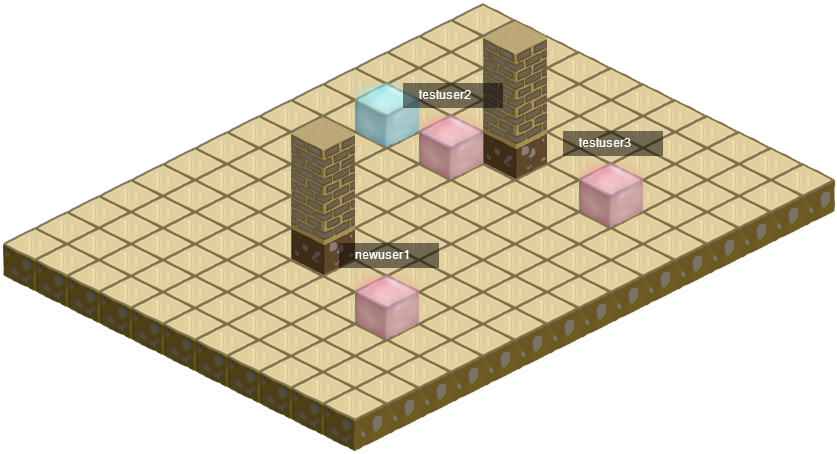
\includegraphics[width=10cm]{Images/the_game.png}
    \caption{The game. Graphics from \cite{GameArt}.}
    \label{fig:the_game}
\end{figure}

Games are interesting projects to take on; they have a history of being difficult to make and pushing technology to its limits. There are a great many systems and features that can be included in them---AI, physics, graphics, audio, UI, multiplayer and more---and a great many ways to implement each, from simple to very complicated depending on the needs of the project.

Games also have a history of aiming for too many of these features in too little time. In most cases, every one of the features thought up would enhance the final product in some way, from a significant improvement that changes the way the game is played to a minor enhancement that makes things just a little more pleasant for the user. Many of these features may be considered mandatory for the game to be worth making at all. For example, a single-player chess game would probably not be very good if there were no AI to play against.

It is clear that, given the sheer enormity of the possible things that can be put into any one game, there is not enough time in this project to implement even half of them without a great deal of previous experience and skill. Every one of the major systems mentioned can be extremely complicated, requiring a lot of research, time and effort to make them work.

This chapter will discuss what the project is; why it was worth taking on; how a minimal system was devised that would satisfy enough of the game design requirements to be playable but also be implementable in the time given; and finally the process used to implement the design requirements.

\section{Background}

\subsection{The Project}
Before discussing the decisions made about what was doable and why it was interesting, it's useful to know what the project actually is.

The name of the project---\textit{Browser-based Online Multiplayer Roleplaying Game}---gives a relatively good hint of the nature of the game. ``Browser-based'' and ``multiplayer'' are fairly self-evident in meaning: multiple people play together in a game hosted in the browser. ``Roleplaying game'' is more ambiguous. In this case, it refers to a game in the style of the classic tabletop roleplaying game \textit{Dungeons \& Dragons.}

In the context of the project that meant the following things: firstly, there needed to be two types of players---regular players and a Game Master. A regular player plays the game as a character inhabiting the world they happen to be in. For example, they may be a dwarf in a fantasy kingdom, or a space marine on a futuristic space station.

The Game Master is a player responsible for building the world, telling the story and controlling characters that aren't controlled by the other players (known as Non-Player Characters or NPCs). Traditionally, the Game Master would also be responsible for enforcing the rules of the world. However, in this project the game was to be responsible for that instead, with the Game Master given the option of overriding or changing the rules if he or she wished to do so.

Combat is the most obvious area where the game enforcing the rules comes into effect. Combat is turn-based, with players put onto a grid and given limits on the distance they can move and number of actions they can perform in each turn. When they attempt to do something---such as attack another character or creature or escape from a trap---they have to roll dice, the result of which decides whether they were successful or not, and how well they succeeded or failed. As an example, a player failing to attack a creature with their sword could simply miss, or they could throw the sword away accidentally, depending on the result of the dice roll.

In the above scenario the dice rolls would be simulated by the game, rather than physical dice being used by the players. The game will also decide whether or not an action was valid in the first place. A player hoping to attack a creature with their sword would be unable to do so if the creature was too far away from them.

The design also called for interactions outside of combat. For instance, a player might be faced with a locked door. To get through a player could attempt to use a key they found or, alternatively, they could attempt to bash the door open with an item, such as an axe, or even their bare hands.

There are a few specific implementation details as well. Apart from the game being played via a browser, there needed to be graphics and those graphics needed to be \textsc{2d} isometric tiles. Further, the server was to be written in Python with the goal of gaining experience in the language.

With this overview of the game it is now important to answer why the project was worth doing.

\subsection{Why Make The Game?}
The first answer to this is that games are interesting in general. Most obviously, the final product of a game is (hopefully) something fun to play with appeal to a wide range of people. More relevant to the context of a project, however, is that games are interesting from a software perspective.

Games are made up of a lot of different parts, each one potentially being difficult to implement by itself. In this game, the most challenging individual parts are graphics and multiplayer. More important than just the individual parts, however, is making sure they integrate properly. In most cases the game needs to share data between these different pieces---game logic needs to know what an object is doing so it can perform game functions on it; the renderer needs to know what the object is doing so that it can be drawn to the screen correctly; the networking part needs to know what the object is doing so that it can forward on any relevant information to the server.

The game also offers a lot of extendibility. Given more time, more features can be added. Each feature, and fitting it together, offers a lot of potential for learning as well. For example, an extra feature could be AI, which is an interesting area in itself that offers a lot of opportunity to learn something new.

\subsection{Reading and Research}
Most of the research in the gaming world is very much a closed source, commercial affair. Being on the cutting edge of games is expensive work, requiring smart people spending a lot of time squeezing everything they can out of technology, plus a whole bunch of people to make content for the technology to show.

Even with the explosion of `indie' games made by one person or a very small team that exist these days, most of them are still closed source and commerical. Even free games are rarely free (and certainly not open source)---existing as a vehicle for microtransactions, asking people to buy consumable cosmetic items or in-game advantages, such as speeding something up, for a small fee.

Of course open source games do exist, though they are relatively rare and not very well known. One of the open source games with most relevance to this project is Mozilla's \textit{BrowserQuest}\cite{citeulike:13139186, citeulike:13139189, citeulike:13139194}, a multiplayer role-playing game created in 2012 to show off the capabilities of modern browsers. It has a few properties that are useful to know for this project, the main one being multiplayer.

However, despite the theoretical usefulness of having access to the source code, it was not as useful in practice as might have been desired or expected. Without documentation that describes the more high level structure of the code it is difficult to read through and understand properly without spending a lot of time on it.

The need to have a higher level overview of structure and concepts leads to books, articles and tutorials.

One of the most popular books available for this is \textit{Game Coding Complete}\cite{citeulike:12394552}. It is a lengthy book but covers a lot of things, both high level and code-specific. Most of the implementation details given are inappropriate for this project because they are for \textsc{3d} graphics, C++ and cover a lot of things like custom memory management that have no equivalent or purpose in a much more simple \textsc{2d}, browser-based game written in JavaScript. However, the high level aspects of game engine design the authors talk about are very useful.

The other major book that was found to be useful in this project is a free book currently available online called \textit{Game Programming Patterns}\cite{citeulike:13049596}. This book describes many common design patterns used in game programming, some being game specific and others being more well known patterns but applied to game programming, such as the classic Factory pattern. Some of the patterns when put together describe a more general structure, in a way similar to \textit{Game Coding Complete.}

The content of these two books informs a great deal of the design that was settled on for this project, with particular emphasis on the central game loop and the event manager. These two fundamental parts of the design act as the glue for the more specific aspects of the code, like the graphics renderer or input manager.

Some other books were also investigated, mostly pertaining to the more specific implementation details of the project such as \textsc{html5} browser games. Two books were found in this area, one which talked about implementation details in \textsc{html5}\cite{citeulike:13000145} and one which did the same thing but with the addition of a focus on isometric graphics\cite{citeulike:13000170}.

These books were less useful than the previous two mentioned, however; they didn't offer much extra for structure and the majority of the code in the project is fairly platform independent and easily transferable to other languages. Where the platform is relevant, the \textit{Mozilla Developer Network}\cite{citeulike:13151262} offers up-to-date APIs that are much easier to search through than a book.

An online resource which proved to be very useful was a tutorial on how to render isometric tiles in games in a simple way\cite{citeulike:13139216}. This tutorial was referenced heavily in early development to get the renderer up and running, but was later adjusted to account for more advanced rendering needs.

Finally, other than the \textit{Mozilla Developer Network,} there were APIs referenced for the various languages and libraries used in the project, which will be introduced in Chapter 3.

\section{Analysis}
With the knowledge that the scope of games can expand to encompass a ridiculous area, and that everything within that scope is likely to be time consuming to implement, it is important to define what features are absolutely mandatory for the game to be worth making, and figure out how long it might take to implement them. This section lists the features chosen for the minimal system and how they were decided upon.

\subsection{Necessary Features}
The first of the necessary features is graphics. Graphics are the player's view into the world, letting them see the state of the game and figure out what their input needs to be. Without this view the only way to see into the world would be to debug the code as it was playing, which is not a very efficient or pleasant way to play a game. Of course, it is reasonable to operate a game with a textual interface; however, the game design specified that graphics be implemented and that those graphics be isometric tiles.

Players will need a way to interact with the game. There are two things that affect how this works: the Game Master and the isometric graphics. The Game Master needs to be able to select different characters to control and, in theory, create maps for the other players to play the game in. Using simple keyboard controls probably wouldn't work very well in this case. Isometric graphics also cause issues with keyboard controls. Players attempting to move their character using, for example, the arrow keys on the keyboard might find themselves confused as to which direction their character will move.

The solution to both of these is mouse-based interaction. The Game Master will be able to click to select characters he wants to control and place tiles and items into the world, and movement will be a case of clicking on the desired location and letting the character move there by itself, so that there is no confusion about direction. The disadvantage to this is that mouse interaction is more complicated to handle than keyboard interaction. With a keyboard you check whether a key is pressed and perform an action based on that. With a mouse you have to work out the location of the cursor and what else is in that location. Further, mouse-based movement requires pathfinding, which ultimately adds another required feature.

The game also requires multiplayer. All interactions in the game happen between players, be they regular players or the Game Master. Without any way for them to interact the game is relatively pointless to play---all you'd get as a player is being able to walk around a map with your character.

Multiplayer implies a few things. The first is that there needs to be a way of clients communicating with some remote version of the game. This could, in theory, be a peer to peer connection, but there are problems with this. The first is that peer to peer is not such an easy thing to support technologically with a browser, as the web operates on a client-server model. The second problem with peer to peer is that there is no trustworthy version of the game. All the players need to have a view into the same world and the underlying data needs to be consistent between them or problems would occur. There is nothing to stop any one of the players from modifying their client to perform actions they shouldn't be able to do, and it being run in a browser using JavaScript makes this even more of an issue as all browsers come with easy access to JavaScript debuggers. A single client could be made the authoritative version (with the Game Master being the most logical choice here). However, if that client is tampered with it would affect the game for everyone.

A server solves both of the issues that peer to peer represents. It is, of course, more natural for a browser to operate in a client-server manner. A server is also far more trustworthy than any individual client, and can be used as an authoritative base for the game so that, even if a player tampers with their client, the other players won't be affected. The disadvantage to a server is that it requires resources and time to host and keep running. The more people who decide to play the game, the more server power is required. If the servers went down, no one would be able to play at all.

These things represent technical requirements as much as game design requirements. Their existence requires consideration in designing the structure of the game code. However, there are some other features required which could be considered purely game design issues.

The first of these is combat. In this case, combat is what makes the game a game. Without it players really only get to walk around a world together and look at how pretty it may or may not be, depending on the quality of the graphics used. The full design of combat is fairly comprehensive and involves a lot of possible things. In the game design overview the idea of levels of success or failure was introduced, with things like throwing away a weapon if a character fails really badly on a dice roll. The game checking for valid options was also required, with the example given being whether a player was close enough to hit another character with a weapon. However, in the full game design there is also the option for ranged attacks using projectiles.

These options all make the game a lot more interesting. However, things like being able to throw away a weapon, or even just having levels of failure, require extra implementation time. It was decided that the project only needed to implement a very basic version of combat with other things considered extras to be done given more time. This basic version of combat was binary success or failure based on dice rolls; only `mêlée' combat, requiring characters to be next to each other; and no items would be implemented in the base game, so no weapons and all combat would essentially be unarmed. This would allow players to fight in the game, which is an important aspect of the game design, without creating too much work adding extra features that need a lot of development time and testing, such as projectiles or the use of items.

There should also be some way of interacting with the world outside of combat. Ideally these interactions would be almost limitless and allow the Game Master to specify even more based on items they add to the game. However, this is also a huge task. Because of the time consuming nature of adding interactions to the game only a few very basic ones should be included into the minimal system.

Finally, the last feature that is considered to be required in a minimal version of the game is a chat system. This is important because the game is multiplayer and operates through players interacting with each other. It is unreasonable to rely on players to have a third party tool available for communication, so some way for them to communicate must be provided by the game. In this case, a simple chat system is the most logical choice as it is not too difficult to implement. The basic version of the chat will be global for the game but an enhanced version could allow local chatting between players who are in a specific area or private messaging between the Game Master and a player if the GM wants to do something special.

% Taking into account the problem and what you learned from the background work, what was your analysis of the problem? How did your analysis help to decompose the problem into the main tasks that you would undertake? Were there alternative approaches? Why did you choose one approach compared to the alternatives?

% There should be a clear statement of the objectives of the work, which you will evaluate at the end of the work.

% In most cases, the agreed objectives or requirements will be the result of a compromise between what would ideally have been produced and what was felt to be possible in the time available. A discussion of the process of arriving at the final list is usually appropriate.


\section{Process}
With a minimal system decided on the task becomes to decide how the time available is to be divided up between each feature and the systems necessary to support them.

The original process chosen was a custom variation of SCRUM, with many of the roles and tools taken out due to the project having just a one-person team. Primarily, this was chosen due to familiarity from an industrial year. There were some potential advantages to the process other than this, however: a minimal system was known and the functionality of each feature was well described from an end user's point of view, which translates well to the idea of SCRUM user stories.

The issue with this process was that, although the features were well understood in regards to their intended functionality, there was no complete understanding of how to implement them. This meant that a lot of time was needed to prototype and gain understanding of the problem area and what would be required to solve it.

The biggest example here was the structure of the code---the game engine that holds all the discrete features together and allows them to share the data they need to work. Initial research had come up with very little of how to realistically do this and much time was spent in the beginning of the project implementing, gaining understanding and then scrapping and reimplementing this fundamental part of the code. Indeed, this pattern would prove relatively true for all the features, though less extreme.

The issue this caused was that underneath each story in the SCRUM process are specific implementation tasks that are tracked. Because the implementation kept changing as the problem became better understood and the solutions improved, these tasks quickly became out of sync with what was actually occurring. The tasks began to follow the implementation, rather than the implementation following the tasks.

To deal with this wasted time, the process was transformed to do away with specific tasks. Rather, the already existing feature list was simply taken and followed in order of priority, with priority based on the understood difficulty of the feature---an area where previous research was more useful and accurate. Features were assigned to a sprint and considered to either be complete or incomplete. The completeness of a feature was decided based on its description in the minimal system specification.

This simplification dramatically reduced the administrative overhead of the process. There remained a way to keep track of what features were done and were still to do and gave a clear idea of what the current task was overall, without having to spend time writing down what the tasks specifically should be in detail, letting the dynamic and evolving nature of the implementation happen freely. The disadvantage was that there was no way to clearly point out how complete a feature was to someone else. This disadvantage was not a huge issue because the team only consisted of one person, who knew what rough level of completeness the active feature was at anyway. However, were the team to become larger this process would need adjustment to communicate task progress more effectively.

% You need to describe briefly the life cycle model or research method that you used. You do not need to write about all of the different process models that you are aware of. Focus on the process model that you have used. It is possible that you needed to adapt an existing process model to suit your project; clearly identify what you used and how you adapted it for your needs.